\begin{figure*}[ht]
  \centering
  \begin{subfigure}[b]{0.3\textwidth}
    \centering
    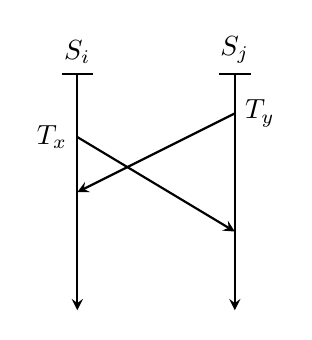
\begin{tikzpicture}
      \draw [thick] (1.3,3) -- (1.7,3);
      \draw [thick,<-,>=stealth] (1.5,0) -- (1.5,3) node[anchor=south] {$S_i$};
      \draw [thick] (3.3,3) -- (3.7,3);
      \draw [thick,<-,>=stealth] (3.5,0) -- (3.5,3) node[anchor=south] {$S_j$};
      \draw [thick,<-,>=stealth] (1.5,1.5) -- (3.5,2.5)  node[right] {$T_y$};
      \draw [thick,->,>=stealth] (1.5,2.2) node[left] {$T_x$} -- (3.5,1);
    \end{tikzpicture}
    \caption{}
    \label{fig:tx-ty}
  \end{subfigure}%
  \begin{subfigure}[b]{0.3\textwidth}
    \centering
    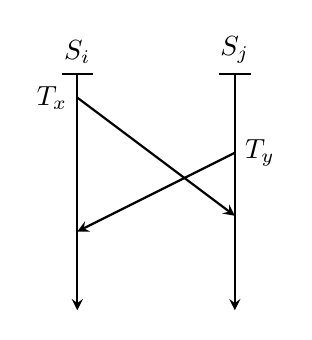
\begin{tikzpicture}
      \draw [thick] (5.3,3) -- (5.7,3);
      \draw [thick,<-,>=stealth] (5.5,0) -- (5.5,3) node[anchor=south] {$S_i$};
      \draw [thick] (7.3,3) -- (7.7,3);
      \draw [thick,<-,>=stealth] (7.5,0) -- (7.5,3) node[anchor=south] {$S_j$};
      \draw [thick,<-,>=stealth] (5.5,1) -- (7.5,2)  node[right] {$T_y$};
      \draw [thick,->,>=stealth] (5.5,2.7) node[left] {$T_x$} -- (7.5,1.2);
    \end{tikzpicture}
    \caption{}
\label{fig:ty-tx}
  \end{subfigure}%
  \begin{subfigure}[b]{0.3\textwidth}
    \centering
    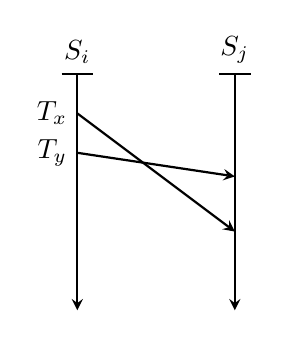
\begin{tikzpicture}
      \draw [thick] (9.3,3) -- (9.7,3);
      \draw [thick,<-,>=stealth] (9.5,0) -- (9.5,3) node[anchor=south] {$S_i$};
      \draw [thick] (11.3,3) -- (11.7,3);
      \draw [thick,<-,>=stealth] (11.5,0) -- (11.5,3) node[anchor=south] {$S_j$};
      \draw [thick,->,>=stealth] (9.5,2.5)  node[left] {$T_x$} -- (11.5,1) ;
      \draw [thick,->,>=stealth] (9.5,2) node[left] {$T_y$} -- (11.5,1.7);
    \end{tikzpicture}
    \caption{}
    \label{fig:same-side}
  \end{subfigure}%
  \caption{Possible interleavings of concurrent transaction's writes to a distributed edge spanning servers $S_i$ and $S_j$ by transactions $T_x$ and $T_y$. In \subref{fig:tx-ty} $T_y$ begins writing to the distributed edge before $T_x$, in \subref{fig:ty-tx} the converse is true, else they are equivalent. In \subref{fig:same-side} both transactions begin writing at the same server but overlap in the network and arrive out-of-order.}
  \label{conf-scen}
\end{figure*}